\documentclass{scrartcl}
\usepackage[utf8]{inputenc}
\usepackage[english]{babel} % Trennung nach der neuen deutschen Rechtschreibung
\usepackage[utf8]{inputenc}
\usepackage[T1]{fontenc}
\usepackage{lmodern}

\usepackage{amsmath} % Erweiterte Mathematik-Umgebung
\usepackage{amsfonts} % zusätzliche Mathematik-Schrifttypen (v.a. \mathbb für Mengen)
\usepackage{ulem}

\usepackage{graphics}%soll beim Graphiken einfügen hilfreich sein
\usepackage{graphicx}
\usepackage{wrapfig}%lässt Textumflossene Bildeinbindung zu
\usepackage{epstopdf}%soll eps in pdf umwandeln

\usepackage[a4paper, portrait, margin=2.5cm]{geometry}

\titlehead{\centering University of Luxemburg}
\subject{Travaux Pratiques}
\title{Hydrogen Atom}
\subtitle{Gilles Friesinger}
\date{TP Session 19/11/2021}
\author{Louis-Hendrik Barboutie (020157041C)\\ Frederik Ehl (0201719742) \\ Florence Schmerber (0201845640)}

\begin{document}

\maketitle

\clearpage

\tableofcontents

\listoffigures
	
\clearpage

\section{Introduction}

In this seventh TP, we want to determine the so called Balmer series, the spectral line emissions of the hydrogen atom. It is characterized by the transition of electrons from the $n\geq3$ to $n=2$ (n is a quantum number). Some spectral lines have special names, like H$_{\alpha}$ form n=3, H$_{\beta}$ for n=4 and H$_{\gamma}$ fro n=5. The relation between the wavelength and the transition of the electron from a higher energy level to a lower energy level is given by the following equation:

\begin{equation}
   \frac{1}{\lambda}=R \cdot (\frac{1}{2^2}-\frac{1}{n^2}) \nonumber
\end{equation}

R being the Rydberg constant, that we will also determine experimentally.
%the main goal of the first part of this experiment is to measure the (lattice parameter/joint fissures per mm/slits) and compare it with the value given by the constructor. In order to do so, we first calibrate our device and then find the deviation angle of the first and second spectrum line...."of the telescope for which we can observe the maxima of the diffraction pattern of the sodium lamp"
%for the second past of this experiment, we want to find experimentally Rydberg's constant. We start by switching the sodium lamp with the hydrogen one and finding out the the angles for which we could observe red, violet and cyan light.
\section{Experimental setup}

We have at our disposal a sodium and a hydrogen lamp, a collimator, the grid and a telescope. 
The light is split into it's different diffraction orders by the grid. The telescope can be moved in order to read the diffraction angles and thus determining the different wavelength.


\begin{figure}[h]
    \centering
    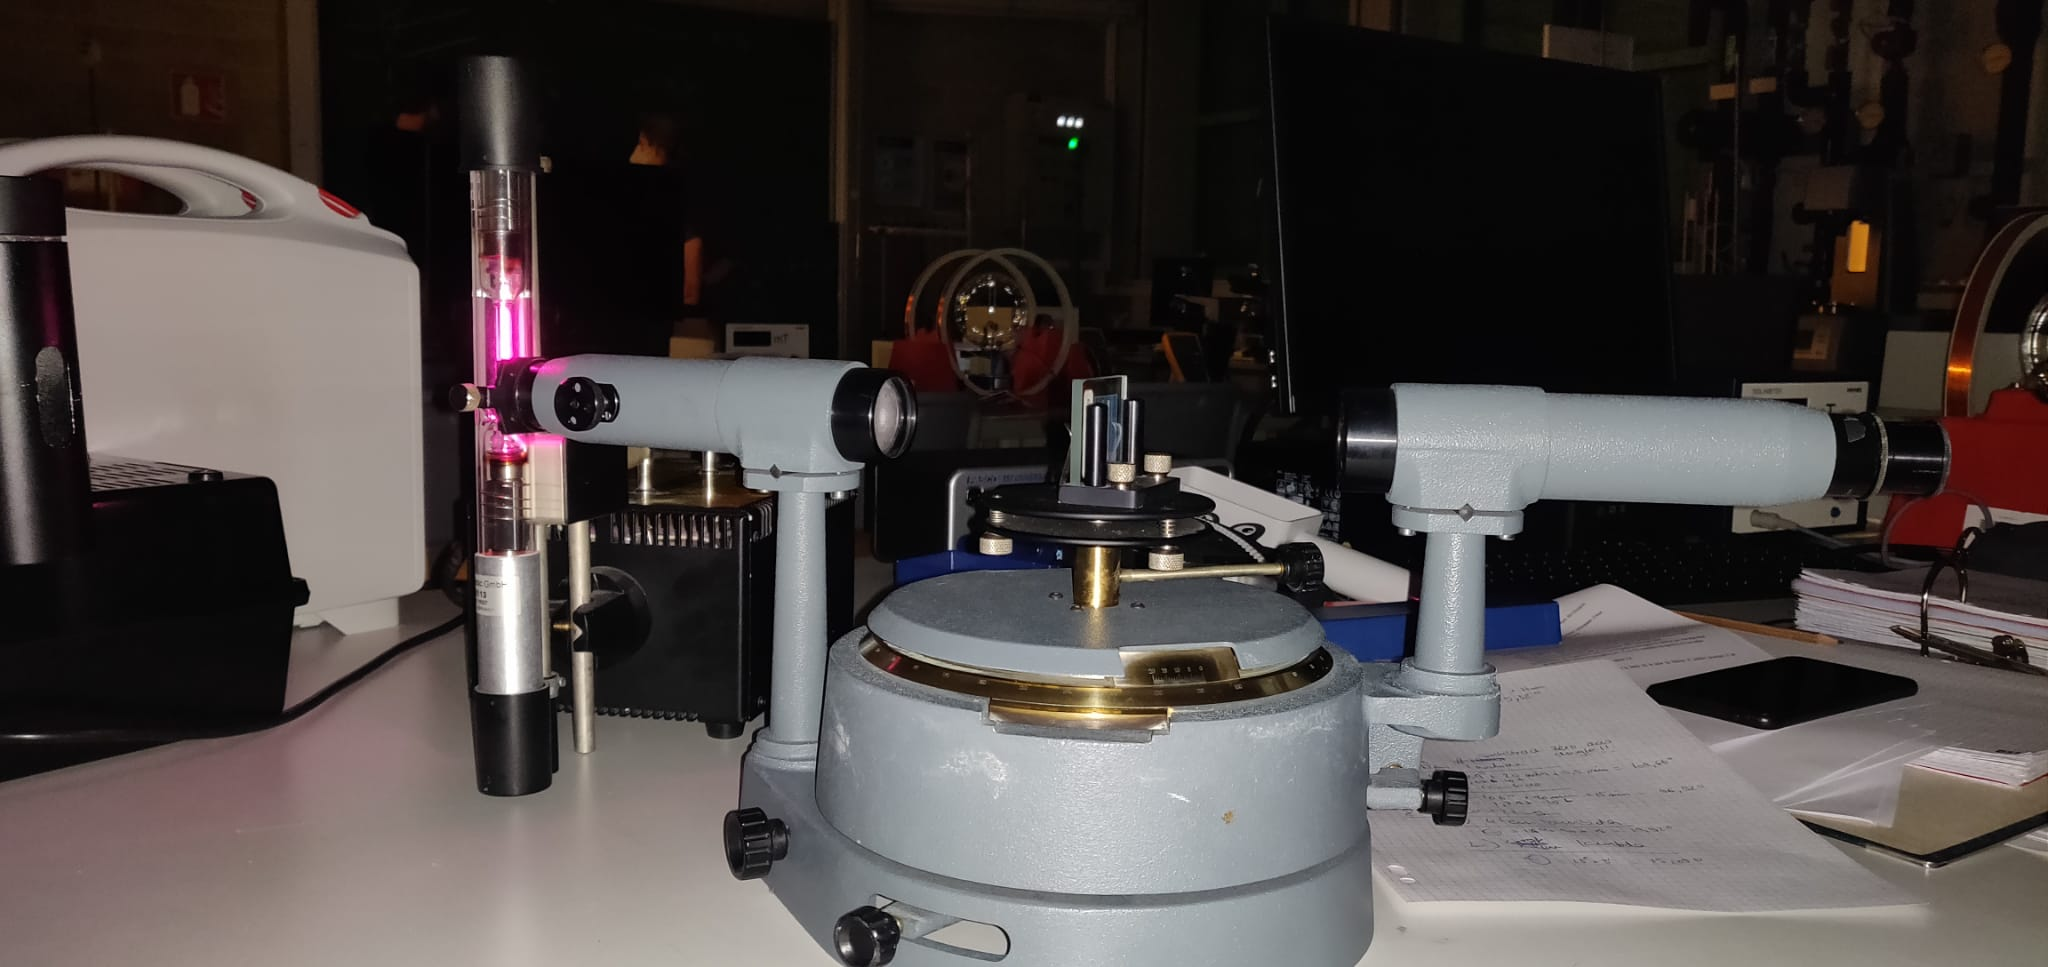
\includegraphics[scale=0.2]{TP7_ExSetup.jpeg}
    \caption{Experimental Setup Hydrogen Lamp}
    \label{fig:2}
\end{figure}


\section{Preliminar Preparation}

In order to get the most precise results in this experiment, we have to properly prepare the experimental setup.
We first calibrate the telescope by focusing an object at infinity. Then we align the telescope with the collimator and note this angle as zero. Going from this angle zero we move the telescope, so that it is at an angle of exactly 90° to the collimator. Afterwards we take the grid and screw it onto the rotatable table. We rotate it until is is at 45° to both the telescope and the collimator, the position where we can observe the light trough the telescope. After having determined the 45° position, we add 45° to it, so that finally the grid is perpendicular to the collimator. 

\section{Results}

\subsection{Determination of the step and the number of slits of the grid}

In the first part of the experiment, we rotate the telescope around the grid and note the angles for which we can observe the maxima of the diffraction pattern of the sodium lamp.The maxima of the pattern are of second order. With the angles that we measure we can calculate the step a between two slits of the grid using the relation:

\centering
\begin{equation}
    a=\frac{k\cdot \lambda}{sin(\theta)}
\end{equation}
\flushleft

The uncertainty is then given by:

\begin{equation}
    U(a) = a_{exp}\sqrt{\frac{U(\theta)^2}{\theta_{exp}^2}}
\end{equation}

Where k is the order of the pattern and the diffraction angle $\theta$ is obtained by the equation:

\centering
\begin{equation}\nonumber
    \theta=\frac{\phi_g-\phi_d}{2}
\end{equation}
\flushleft

The uncertainty is then given by:
\begin{equation}
    U(\theta)= \sqrt{\frac{1}{2^2}U^2(\theta_{g,exp})+\frac{1}{2^2}U^2(\theta_{d,exp})}
\end{equation}

Since the maxima of the pattern are of second order, we observe two spectral lines. We note the angles for both spectral lines.
We note $\phi_g$, the angle we measured on the left side of the zero axis and $\phi_d$ the angle, we measured on the right side of the zero axis.
For the wavelengths we use the values given by the script, $\lambda_1=589,0nm$ and $\lambda_2=589,6nm$.\newline

We have an uncertainty of $30"$ on the reading of the angular position. For calculation purposes we convert it into degrees, for which we obtain $0,00833^\circ$. We choose to enlarge the error to $0,01^\circ$. Furthermore we assume the uncertainty on the wavelengths of the sodium spectral lines to be negligible.
 

\medskip
\centering
\begin{tabular}{|c|c|c|c|c|}
    \hline
     &$\phi_g (^{\circ})$ & $\phi_d(^{\circ})$ & $\theta(^{\circ})$ & $a (10^{-6}m)$\\
     \hline
     $1$ & $194,92\pm 0,01$ & $104,66\pm 0,01$ & $45,13\pm 0,01$ & $1,644 \pm 0,03$\\
     \hline
     $2$ & $195,05\pm 0,01$ & $106,92\pm 0,01$ & $44,07\pm 0,01$ & $1,696 \pm 0,03$ \\
     \hline
\end{tabular}
\flushleft

We obtain an average step of $a_{average}=1,67\mu m$. We can calculate the number of slits of the grid per millimeter length with $N=\frac{1}{a}$. We obtain an average of $N=595mm^{-1}$. Compared with the value given by the manufacturer of $N=600mm^{-1}$, we obtain an error of approximately $0,83\%$.


\subsection{Verification of the Balmer series produced by the Hydrogen Atom}
For the following we replace the sodium lamp with the hydrogen lamp. We repeat the measuring process as before for each line we observe in the spectrum. Note that there were some impurities in the lamp, so we also observed lines for different elements, ie. some orange and green lines. In order to determine the wavelength $\lambda$ of the emitted spectral lines we use the relation:

\begin{equation} \nonumber
    \lambda = \frac{a\cdot sin(\theta_k)}{k}
\end{equation}
which reduces to
\begin{equation}
    \lambda = a\cdot sin(\theta)
\end{equation}
since the observed spectral lines are of first order.

The uncertainty is then given by:
\begin{equation}
    U(\lambda)= \lambda_{exp}\sqrt{\frac{U^2(a)}{a^2_{exp}}+\frac{U^2(\theta)}{\theta_{exp}}}
\end{equation}

We got following values for the spectral lines of hydrogen:

\medskip
\centering
\begin{tabular}{|c|c|c|c|c|c|}
    \hline
     & $\phi_g (^{\circ})$ & $\phi_d (^{\circ})$ & $\theta(^{\circ})$ & $\lambda (nm) $ & Colour \\
    \hline
    1 & $344,53 \pm 0,01$ & $314,28\pm 0,01$ & $15,13\pm 0,01$ & $435,75 \pm 0,29$ & Dark blue \\
    2 & $346,75\pm 0,01$ & $312,02\pm 0,01$ & $17,37\pm 0,01$ & $498,43 \pm 0,29$ & Teal \\
    3 & $352,93\pm 0,01$ & $306,10\pm 0,01$ & $23,42\pm 0,01$ & $663,64 \pm 0,29$ & Red \\
    \hline
\end{tabular}
\flushleft

We now compare the obtained wavelengths for the Balmer series produced by the hydrogen atom with the literature values and calculate the relative error, in order to determine the precision of the experiment.

\medskip
\centering
\begin{tabular}{|c|c|c|c|c|}
    \hline
     Transition of n & Color & $\lambda_{exp}(nm)$ & $\lambda_{th}(nm)$ & relative error\\
     \hline
     $5\rightarrow2$ &Dark blue & $435,75$ & $434,05$ & $0.39\%$ \\
     \hline
     $4\rightarrow2$ & Teal & $498,43$ & $486.15$ & $2.52\%$ \\
     \hline
     $3\rightarrow2$ & Red & $663,64$ & $656,27$ & $1.12\%$ \\
     \hline
     
\end{tabular}
\flushleft

\subsection{Determination of the Rydberg constant}
We can also use our data to determine the Rydberg constant, using the relationship:

\begin{equation}
    f(\lambda) = \frac{1}{\lambda} = R \cdot (\frac{1}{p^2}-\frac{1}{n^2})
\end{equation}

Where $n=3,4,5$ and $p=2$. The red wavelength corresponds to n=3, the teal wavelength to n=4 and finally the dark blue wavelength to n=5.

\begin{figure}[h]
    \centering
    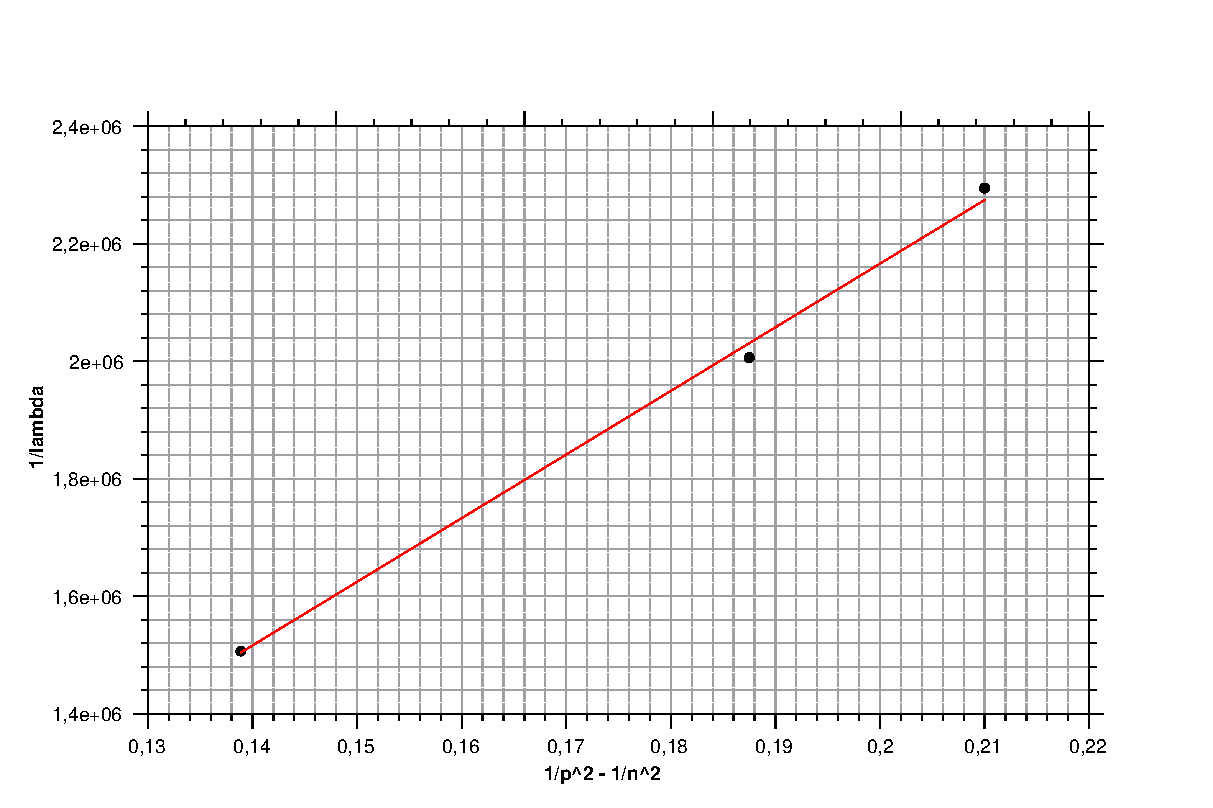
\includegraphics[width=12cm]{TP7_RydbergCst.eps}
    \caption{Graph of $f(\lambda)$}
    \label{fig:my_label}
\end{figure}

\newpage

The slope of the linear fit is the Rydberg constant as seen in equation (2).
Thus the experimental value for the Rydberg value is $R_{exp}= (1,083 \pm 0,008) \cdot 10^7 \ m^{-1}$. We can determine the relative error to the theoretical value by:
\begin{equation}
    \frac{|R_{th}-R_{exp}|}{R_{th}} \cdot 100 \approx 1,28\%
\end{equation}

\subsection{Limit of the Balmer series}
If we consider the limit of the Balmer series, which means that $n\rightarrow \infty$ , the relation (2) ends up to be:
\begin{equation}
    \frac{1}{\lambda} = R_{exp} \cdot (\frac{1}{p^2})
\end{equation}
Where here p=2.
We get for the wavelength $\lim_{n \to \infty}(\lambda_n)=369,3nm$.
Knowing that the visible range of light is usually between 380nm and 780nm, we can conclude that we cannot see this spectral line.

\section{Conclusion}
In this series of experiments we were able to determine the the step and the number of slits of the grid we worked with. We could verify the Balmer series produced by the hydrogen atom and thereby determine the Rydberg constant experimentally. The results we obtained are satisfying even though the literature values of the wavelengths were outside of our uncertainty brackets.
\end{document}